
\serie{Thèorème de Pythagore}

\begin{exercice}[]
On considère le  parallélogramme STOP dessiné à main levée.\\
\begin{minipage}{0.55\linewidth}


Démontrer que le parallélogramme STOP est un rectangle.

\end{minipage}
\hfill
\begin{minipage}{0.4\linewidth}
\begin{center}
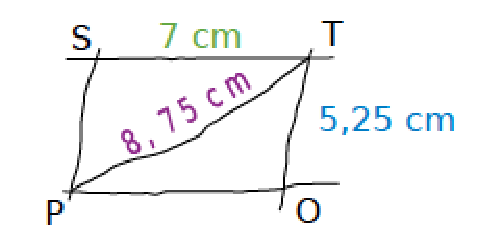
\includegraphics[scale=0.45]{GP1}
\end{center}
\end{minipage}
\end{exercice}


\begin{exercice}[]
Sur la figure ci-contre :

\begin{minipage}{0.6\linewidth}
\begin{itemize}
\item EFGH est un rectangle ;
\item EF = 14 m \emph{et} FG = 12 m ;
\item K $\in$ [EH] \emph{et} EK = 4 m ;
\item L $\in$ [EF] \emph{et} EL = 6 m.
\end{itemize}
Le triangle KGL est-il rectangle ?

\end{minipage}
\hfill
\begin{minipage}{0.35\linewidth}
\begin{center}

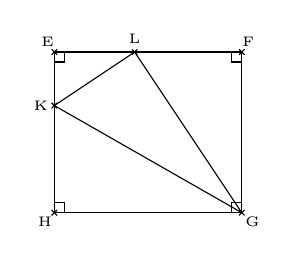
\begin{tikzpicture}[x=0.17cm,y=0.17cm]
\draw[fill=black,fill opacity=0] (0.7415589313755807,0.0) -- (0.7415589313755808,0.7415589313755807) -- (4.540738858441183E-17,0.7415589313755807) -- (0.0,-0.0) -- cycle; 
\draw[fill=black,fill opacity=0] (13.25844106862442,12.0) -- (13.25844106862442,11.25844106862442) -- (14.0,11.25844106862442) -- (14.0,12.0) -- cycle; 
\draw[fill=black,fill opacity=0] (4.540738858441183E-17,11.25844106862442) -- (0.7415589313755808,11.25844106862442) -- (0.7415589313755807,12.0) -- (0.0,12.0) -- cycle; 
\draw[fill=black,fill opacity=0] (14.0,0.7415589313755807) -- (13.25844106862442,0.7415589313755808) -- (13.25844106862442,9.081477716882366E-17) -- (14.0,0.0) -- cycle; 
\draw (0.0,-0.0)-- (0.0,12.0);
\draw (0.0,12.0)-- (14.0,12.0);
\draw (14.0,12.0)-- (14.0,0.0);
\draw (14.0,0.0)-- (0.0,-0.0);
\draw (0.0,8.0)-- (6.0,12.0);
\draw (6.0,12.0)-- (14.0,0.0);
\draw (14.0,0.0)-- (0.0,8.0);
\begin{tiny}
\draw [color=black] (0.0,-0.0)-- ++(-1.0pt,-1.0pt) -- ++(2.0pt,2.0pt) ++(-2.0pt,0) -- ++(2.0pt,-2.0pt);
\draw[color=black] (-0.7,-0.7) node {H};
\draw [color=black] (14.0,0.0)-- ++(-1.0pt,-1.0pt) -- ++(2.0pt,2.0pt) ++(-2.0pt,0) -- ++(2.0pt,-2.0pt);
\draw[color=black] (14.8,-0.7) node {G};
\draw [color=black] (0.0,12.0)-- ++(-1.0pt,-1.0pt) -- ++(2.0pt,2.0pt) ++(-2.0pt,0) -- ++(2.0pt,-2.0pt);
\draw[color=black] (-0.5,12.8) node {E};
\draw [color=black] (14.0,12.0)-- ++(-1.0pt,-1.0pt) -- ++(2.0pt,2.0pt) ++(-2.0pt,0) -- ++(2.0pt,-2.0pt);
\draw[color=black] (14.5,12.8) node {F};
\draw [color=black] (0.0,8.0)-- ++(-1.0pt,-1.0pt) -- ++(2.0pt,2.0pt) ++(-2.0pt,0) -- ++(2.0pt,-2.0pt);
\draw[color=black] (-1,8) node {K};
\draw [color=black] (6.0,12.0)-- ++(-1.0pt,-1.0pt) -- ++(2.0pt,2.0pt) ++(-2.0pt,0) -- ++(2.0pt,-2.0pt);
\draw[color=black] (6,13) node {L};
\end{tiny}
\end{tikzpicture}
\end{center}
\end{minipage}
\end{exercice}

\serie{Théorème de Thalès}

\begin{exercice}[]
On suppose que (AB)$\parallel$(CD).

On a AB = 72, CD = 96, SC = 84 et SD = 72.
 
Trouver SA et SB.
\begin{center}
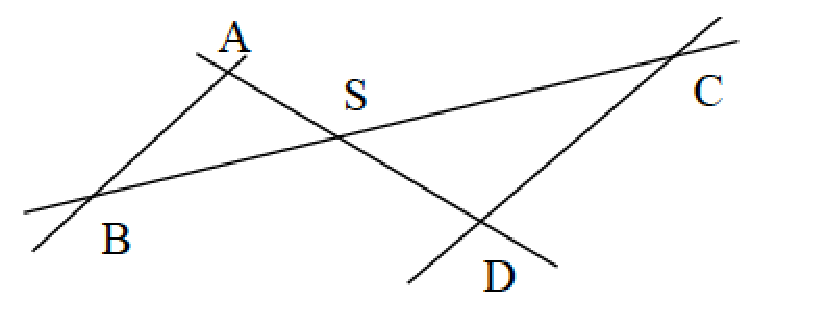
\includegraphics[scale=0.35]{GP2}
\end{center}
\end{exercice}

\begin{exercice}[]
On suppose que (AB)$\parallel$(CD) et que (AB)$\parallel$(EF).
 
AC= 10, CE = 15 et BD = 14.

Trouver DF.
\begin{center}
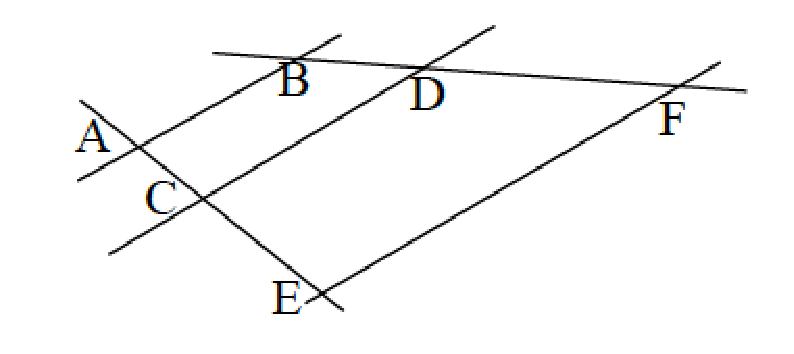
\includegraphics[scale=0.35]{GP3}
\end{center}
\end{exercice}

\begin{exercice}[]
On a : OM = 2,8 cm ; ON = 5,4 cm ; OS = 2,7 cm et OT = 1,4 cm.
Démontrer que les droites (MN) et (ST) sont parallèles.
\begin{center}
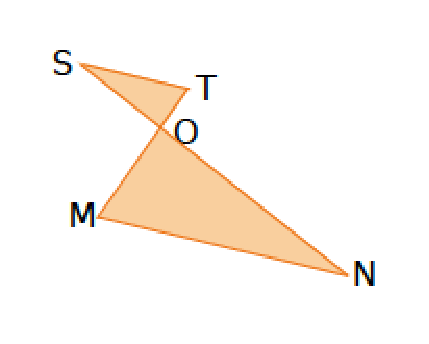
\includegraphics[scale=0.35]{GP4}
\end{center}
\end{exercice}

\begin{exercice}[]
L'unité de longueur choisie est le mètre. 
\begin{center}
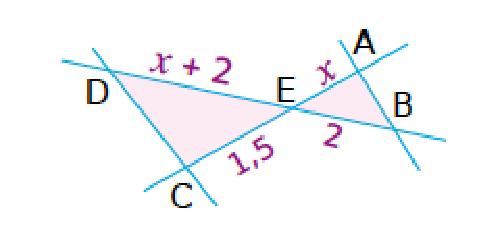
\includegraphics[scale=0.5]{GP7}
\end{center}

\begin{enumerate}
\item Pour $x = 2,5$, les droites (AB) et (CD) ne sont pas parallèles. 
Vrai ou faux? Expliquer la démarche.
\item Pour $x = 1$, les droites (AB) et (DC) ne sont pas parallèles. Vrai ou faux ? Expliquer la démarche.
\end{enumerate}
\end{exercice}

\begin{exercice}[]
Sur ce schéma les droites (EF) et (GH) sont sécantes en D.\\
Les droites (EG) et (FH) sont parallèles.\\
\begin{center}
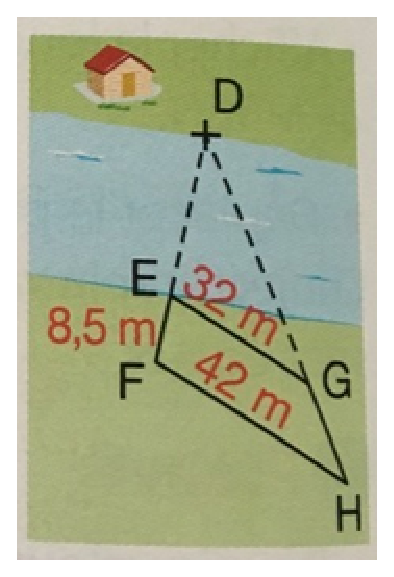
\includegraphics[scale=0.45]{GP10}
\end{center}
Quelle est la largeur DE de la rivière?
\end{exercice}

\serie{Divers}

\begin{exercice}[]
Sur la figure ci-dessous : GR=3,4 cm. 

Le point S est le milieu du côté [GR]. 

Calculer ST. 
\begin{center}
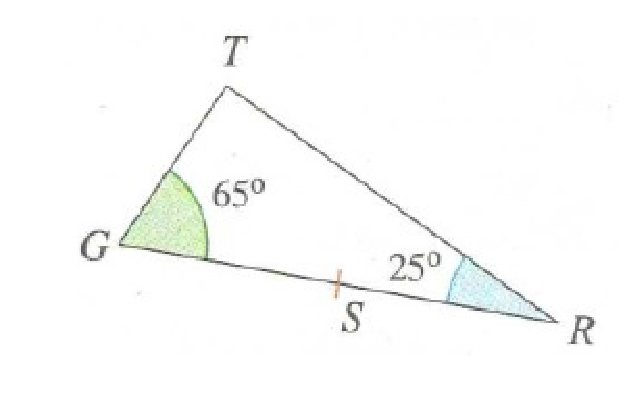
\includegraphics[scale=0.5]{GP5}
\end{center}
\end{exercice}

\begin{exercice}[]
Pour consolider un bâtiment, des charpentiers  ont construit un contrefort en bois (les mesures sont en mètre).

\begin{center}
\includegraphics[scale=0.5]{GP8}
\end{center}

\begin{enumerate}
\item En considérant que le montant [BS] est perpendiculaire au sol, calculer la longueur AS.
\item Calculer les longueurs SM et SN.
\item Démontrer que la traverse [MN] est bien parallèle au sol.
\end{enumerate}
\end{exercice}

\begin{exercice}[]
Sur cette figure, C est un cercle de centre O et de rayon 3 cm.

La droite (d) est tangente en A au cercle C .

On voudrait calculer la longueur en cm du segment [OB].

1) Expliquer pourquoi on peut utiliser le théorème de Pythagore dans le triangle OAB.

2) Calculer l’arrondi au dixième de la longueur OB en cm.
\begin{center}
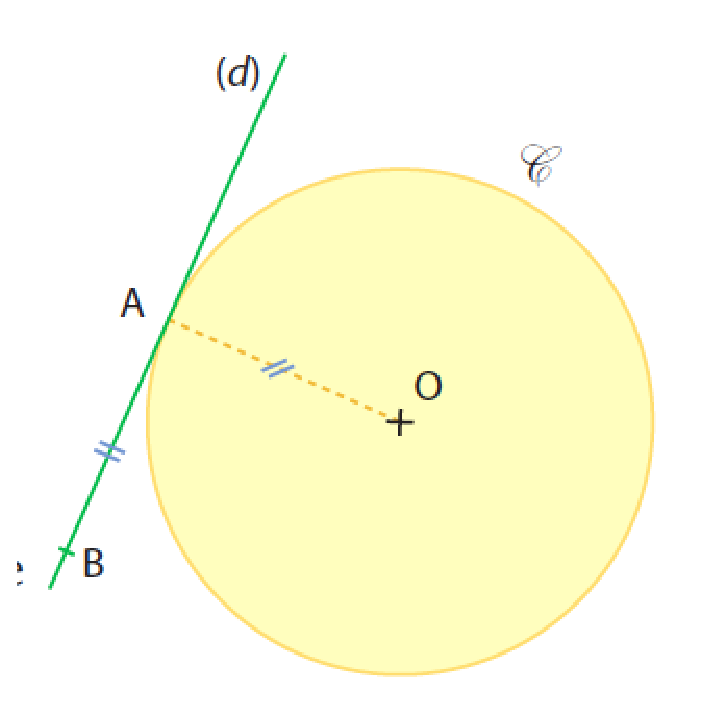
\includegraphics[scale=0.45]{GP6}
\end{center}
\end{exercice}

\begin{exercice}[]
Sur la figure, les droites (EF) et (MP) sont parallèles.
\begin{center}
\includegraphics[scale=0.5]{GP9}
\end{center}

On sait que AM=6 cm ; MP=4,8cm ; AP=3,6 cm ; EF=6 cm ; AC=4,5 cm et AB=7,5 cm .

\begin{enumerate}
\item Démontrer que le triangle AMP est un triangle rectangle.
\item Calculer AE puis la longueur ME.
\item Démontrer que les droites (MP) et (BC) sont parallèles.
\end{enumerate}
\end{exercice}



